% Define document class
\documentclass[twocolumn]{aastex63}
\DeclareRobustCommand{\Eqref}[1]{Eq.~\ref{#1}}
\DeclareRobustCommand{\Figref}[1]{Fig.~\ref{#1}}
\DeclareRobustCommand{\Tabref}[1]{Tab.~\ref{#1}}
\DeclareRobustCommand{\Secref}[1]{Sec.~\ref{#1}}
\newcommand{\todo}[1]{{\large $\blacksquare$~\textbf{\color{red}[#1]}}~$\blacksquare$}
\newcommand{\mr}[1]{{\textbf{\color{green!75!black}[#1]}}}
% \usepackage{cuted}
\usepackage{flushend}
\usepackage{amsmath}
% \graphicspath{{./figures/}}

\begin{document}

% Title
\title{\todo{title}}

\author[0009-0008-2061-4946]{C.~A.~Burt}
\affiliation{University of Arizona, Department of Astronomy \& Steward Observatory, 933 N.~Cherry Ave., Tucson, AZ 85721, USA}

\author[0000-0002-6718-9472]{M.~Renzo}
\affiliation{University of Arizona, Department of Astronomy \& Steward Observatory, 933 N.~Cherry Ave., Tucson, AZ 85721, USA}

\author[0000-0002-2215-1841]{A.~Grichener}
\affiliation{University of Arizona, Department of Astronomy \& Steward Observatory, 933 N.~Cherry Ave., Tucson, AZ 85721, USA}

\author{\todo{TBD}}

\begin{abstract}
  Common phases of mass transfer in stellar binaries are case A
  (during the donor's main sequence) and case B (after the donor's
  main sequence but before helium core depletion). For most masses,
  radii significantly grow after the main sequence, making case B more
  common. However, very massive stars ($\gtrsim 30\,M_\odot$) may
  already undergo significant expansion during the main sequence
  increasing the probability of case A mass transfer, but this depends
  on uncertain stellar physics. For observationally-informed
  convective boundary mixing, case A mass transfer dominates for donor
  masses $\gtrsim 75 \, M_{\odot}$.  This is not the case without
  convective boundary mixing or with the values assumed in rapid
  binary population synthesis. Therefore, case A mass transfer may be
  more dominant than commonly assumed, with potential impact on rates
  of all post mass transfer binaries.
\end{abstract}

\section{Mass Transfer in Very Massive Binaries}

Binary stars with a sufficiently small orbital separation undergo a
mass transfer phase in which one donor star transfers mass to an
accretor. For very massive stars ($ \gtrsim 30 \, M_{\odot}$), mass
transfer most often occurs as case A or case B \cite{kippenhahn:67}.

\begin{figure*}[htbp]
  \centering
  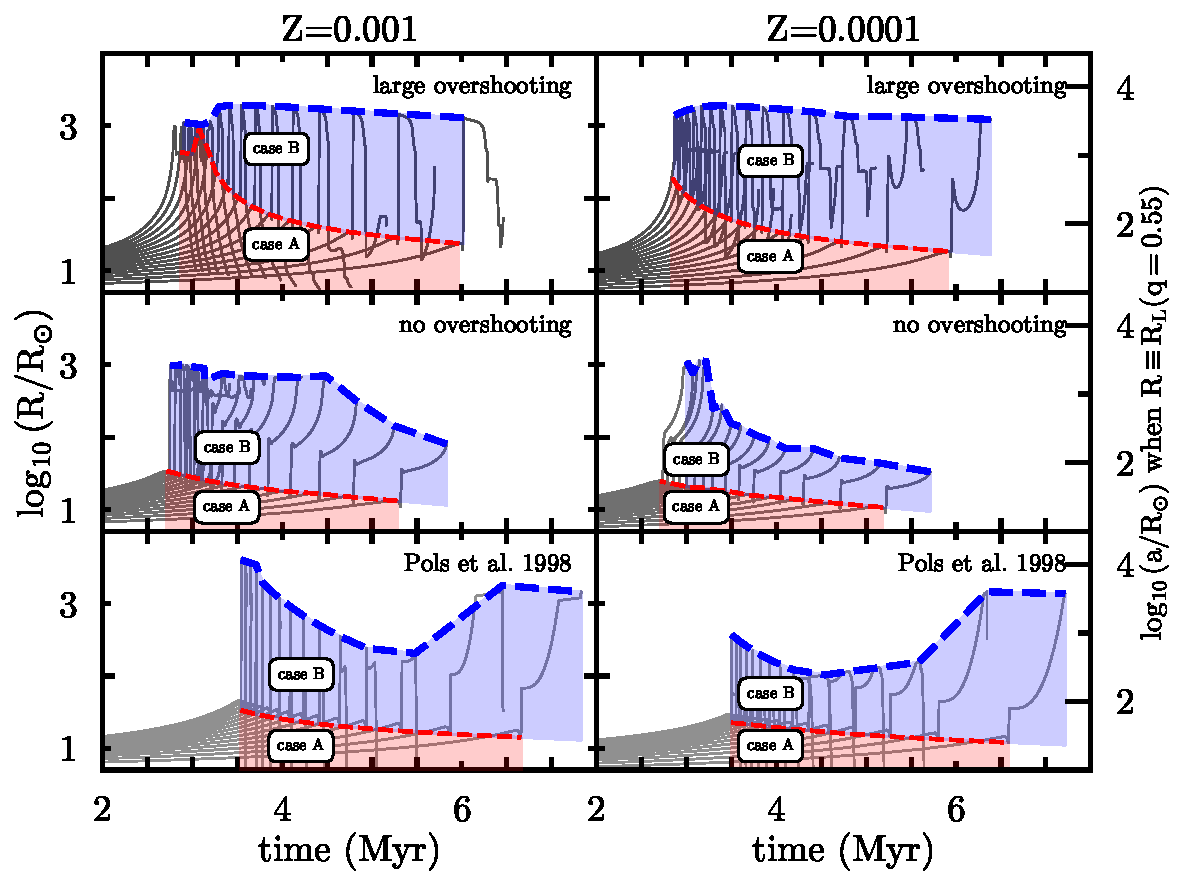
\includegraphics[width=0.9\textwidth]{radii}
  \caption{Each panel contain 15 stellar models spanning from a
    $30 \, M_{\odot}$ star on the right to a $100 \, M_{\odot}$ with
    intervals of width $5 \, M_{\odot}$. The top panels plot models
    that feature broad convective boundary mixing, the middle panels
    plot models that do not feature overshooting, and the bottom
    panels plot models generated from COMPAS using data from
    \cite{pols:98}. The left panels have a metallicity $Z=0.001$ and
    the right panels have a metallicity $Z=0.0001$}
  \label{fig:R_t_donor}
\end{figure*}


Case B is expected more often than case A mass transfer, since stars
in most mass ranges expand most prominently post-main sequence in the
Hertzsprung gap \citep{vandenheuvel:69}. However, very massive stars
may already undergo a drastic expansion in radius during their main
sequence. \citep[e.g.,][]{sanyal:15, jiang:15, sabhahit:24}. This may
increase the rate of case A \citep{demink:08}, which could have
significant implications on the rates of Wolf-Rayet+O-type binaries,
X-ray binaries, and gravitational wave progenitors. The radius of the
donor is dependent on unknown stellar parameters, including stellar
winds \citep{renzo:17, josiek:24}, metallicity \citep{xin:22},
close-to-super-Eddington-layers \citep[e.g.,][]{joss:73, paxton:13,
  jiang: 15}, and convective boundary mixing \citep{anders:23,
  johnston:24}. Here, we illustrate this comparing the radial
evolution of very massive stars varying convective boundary mixing,
metallicity, and models commonly adopted in rapid binary population
synthesis.

\section{}

We computed 60 MESA models (version 24.03.1) from $30 \, M_{\odot}$ to
$100 \, M_{\odot}$ at metallicity $Z=0.001,0.0001$ following the setup
from \cite{renzo:23} with and without overshooting and compared them
to the \cite{pols:98} models used in SSE/BSE \cite{hurley:00} taken
from COMPAS \cite{stevenson:17, vignagomez:18, riley:22}. Individual
models are shown in gray, and the red and blue lines in each panel of
Fig.~\ref{fig:radii} denote the maximum radius during the main
sequence and helium core burning phase respectively. The right axis
shows orbital separations where the stellar radius meets the roche
radius \citep{eggleton:83} considering a typical accretor-to-donor
mass ratio of $q=0.55$. The red regions denote binaries which will
undergo case A mass transfer and the blue regions denote binaries
which will undergo case B mass transfer. In the top left panel, donors
with masses $ \gtrsim 75 \, M_{\odot}$ can only experience case
A. Removing convective boundary mixing (middle) keeps main sequence
radii smaller, preserving the blue region at all masses. The
overshooting implementation from \cite{pols:98} (bottom), while
nonzero, still leaves a large window for case B up to
$100 \, M_{\odot}$. At even lower metallicities (right), stars are
more compact, and all models allow for case B mass transfer at all
masses.

% The relative proportion of case A mass transfer in comparison to case
% B mass transfer scales with mass of the donor star. This is expected,
% as larger stars see greater rates of radial expansion during the main
% sequence. This has a significant side effect for stars
% with($\gtrsim 75M_{\odot}$), case A mass transfer is expected to
% explain in all possible mass transfer processes. For stars of lesser
% mass, the thermal expansion of the star at the end of the main
% sequence expands the star beyond its maximum radius during the main
% sequence. However, for stars in this mass range, the radius expands
% drastically during the main sequence, such that the maximum radius
% during the main sequence and helium core burning phase are similar.

In order to demonstrate the change in ratio between instances of case
A and case B mass transfer, we modelled 60 stars while varying mass
($30-100 M_{\odot}$; of $5M_{\odot}$ intervals), metallicity
($Z = 0.001,0.001$) and model of boundary mixing. The top panels of
FIGURE are determined from the exponential boundary mixing model from
\cite{herwig:00} fit to the expected values from the step boundary mixing
model from \cite{brott:11}. This is configured in
\cite{claret:18}. This ``broad convective boundary mixing'' model is
compared to a model that does not consider boundary mixing. Both
models were instructed to end before the carbon burning phase could
commence.

In addition, 30 models generated using the rapid population synthesis
code COMPAS using models generated from data gathered in
\cite{pols:98} are plotted in the bottom panels of FIGURE. These
models match the metallicities of the stellar evolution models in the
other panels. These models include data until core collapse.

Convective boundary mixing has a strong effect on stellar radius
\cite{brott:11, johnston:24}, which determines Roche lobe
overflow. The vast differences in the ratio of expected abundances of
case A and case B mass transfer are consequentially expected. The
broad convective boundary mixing models limit case B mass transfer for
stars of mass ($\gtrsim 75M_{\odot}$) . In contrast, omitting
convective boundary mixing allows case B mass transfer to occur at a
significant scale in all mass regimes such that $M<100_{\odot}$. HOW
TO CITE Brott's paper suggests broad convective boundary mixing models
currently provide the best approximation for observed characteristics
of massive stars. As a result, many rapid population synthesis
softwares and other stellar mass transfer models may underestimate the
abundance of case A mass transfer procedures.

Binary interactions are crucial to the formation of X-ray binaries and
gravitational waves sources. in particular for BBH stable mass
transfer may dominate \cite{marchant:21, vanson:21}}


\bibliography{./donorR.bib}
\end{document}

%%% Local Variables:
%%% mode: latex
%%% TeX-master: t
%%% End:
